\documentclass[a4paper,11pt]{article}
\usepackage[utf8]{inputenc}
\usepackage[spanish]{babel}
\usepackage[affil-it]{authblk}
\usepackage{enumerate}
\usepackage{graphicx}
\usepackage{listings}
\usepackage{hyperref}
\usepackage{amsmath}
\usepackage{amssymb}
\usepackage{cancel}
\usepackage[usenames, dvipsnames]{color}
\usepackage{tikz}
\usepackage[labelfont=bf]{caption}
\usepackage{subcaption} %Multiple images
\usepackage{multicol} % Multiple columns
\usepackage{float}
\usepackage{cleveref}
\usepackage{relsize} % bigger math symbols
\usepackage[margin=1.1in]{geometry}
\usepackage[titletoc,toc,title]{appendix}
\usepackage{enumitem}
\usepackage{etoolbox}
\usepackage{mdframed} %frame theorems
\usetikzlibrary{calc}
\numberwithin{equation}{section}

% Footnotes with symbols

\makeatletter
\def\@fnsymbol#1{\ensuremath{\ifcase#1\or \dagger\or \ddagger\or
   \mathsection\or \mathparagraph\or \|\or **\or \dagger\dagger
   \or \ddagger\ddagger \else\@ctrerr\fi}}
\makeatother

\renewcommand{\thefootnote}{\fnsymbol{footnote}}

%Styling for code
\definecolor{codegreen}{rgb}{0,0.6,0}
\definecolor{codegray}{rgb}{0.5,0.5,0.5}
\definecolor{codepurple}{rgb}{0.58,0,0.82}
\definecolor{backcolour}{rgb}{0.95,0.95,0.92}
 
\lstdefinestyle{mystyle}{
    backgroundcolor=\color{backcolour},   
    commentstyle=\color{codegreen},
    keywordstyle=\color{magenta},
    numberstyle=\tiny\color{codegray},
    stringstyle=\color{codepurple},
    basicstyle=\footnotesize,
    breakatwhitespace=false,         
    breaklines=true,                 
    captionpos=b,                    
    keepspaces=true,                 
    numbers=left,                    
    numbersep=5pt,                  
    showspaces=false,                
    showstringspaces=false,
    showtabs=false,                  
    tabsize=2
}
 
\lstset{style=mystyle}

% Cool letters 
%Filename:      Typocaps.fd
%Created by:    MLO
%Creation date: 2003/04/02

% This file should be put in a TeX input directory

\ProvidesFile{Typocaps.fd}
   [2003/04/02 Font definition file for U/Typocaps]

\DeclareFontFamily{U}{Typocaps}{}

\DeclareFontShape{U}{Typocaps}{xl}{n}{
   <-> Typocaps
}{}

\endinput


% Footer
\usepackage{fancyhdr}
\pagestyle{fancy}
\fancyhf{}
\cfoot{\fontsize{15pt}{15pt}\usefont{U}{Typocaps}{xl}{n} 
gigantium humeris insidentes}

% Big Pictures
\usepackage[export]{adjustbox}

% Enviroment for theorems
\newmdtheoremenv[frametitle=Teorema]{theo}{Theorem}

% Circled words
\newcommand{\circled}[2][]{%
  \tikz[baseline=(char.base)]{%
    \node[shape = circle, draw, inner sep = 1pt]
    (char) {\phantom{\ifblank{#1}{#2}{#1}}};%
    \node at (char.center) {\makebox[0pt][c]{#2}};}}
\robustify{\circled}

%Appendices in spanish
\renewcommand{\appendixname}{Ap\'endices}
\renewcommand{\appendixtocname}{Ap\'endices}
\renewcommand{\appendixpagename}{Ap\'endices}

%Zero delimiter
\newcommand{\zerodel}{.\kern-\nulldelimiterspace}

%Columns separation
\setlength{\columnsep}{1cm}

%Indentation
\setlength{\parindent}{0ex}

%Multiple References

\crefrangelabelformat{equation}{(#3#1#4--#5\crefstripprefix{#1}{#2}#6)}

\usepackage{xparse}

%Boxes

\newcommand*{\boxcolor}{blue}
\makeatletter
\renewcommand{\boxed}[1]{\textcolor{\boxcolor}{%
\tikz[baseline={([yshift=-1ex]current bounding box.center)}] \node [rectangle, minimum width=1ex,rounded corners,draw] {\normalcolor\m@th$\displaystyle#1$};}}
 \makeatother

%Constantes
\newcommand{\euler}{\mathrm{e}}
\newcommand{\im}{i}

%Lemas, teoremas, definiciones y pruebas
\newcommand{\definicion}{\textbf{Definición: }}
\newcommand{\lema}{\textbf{Lema: }}
\newcommand{\teorema}{\textbf{Teorema: }}
\newcommand{\prueba}{\textbf{Prueba: }}
\newcommand{\proposicion}{\textbf{Proposición: }}
\newcommand{\corolario}{\textbf{Corolario: }}

% Definición de las secciones y su numeración

\makeatletter
\def\@seccntformat#1{%
  \expandafter\ifx\csname c@#1\endcsname\c@section\else
  \csname the#1\endcsname\quad
  \fi}
\makeatother

\begin{document}

\begin{titlepage}
\thispagestyle{fancy}

\newcommand{\HRule}{\rule{\linewidth}{0.5mm}} % Defines a new command for the horizontal lines, change thickness here

\center % Center everything on the page
 
%----------------------------------------------------------------------------------------
%	HEADING SECTIONS
%----------------------------------------------------------------------------------------

\textsc{\LARGE Universidad Nacional Autónoma de México}\\[0.3cm] % Name of your university/college

%----------------------------------------------------------------------------------------
%	LOGO SECTION
%----------------------------------------------------------------------------------------


\includegraphics[scale=0.17]{unam}

%----------------------------------------------------------------------------------------
%	SUBHEADING SECTIONS
%----------------------------------------------------------------------------------------

\textsc{\Large Electrodinámica Clásica}\\[0.3cm] % Major heading such as course name
\textsc{\large Semestre 2016-II}\\[0.3cm] % Minor heading such as course title
\textsc{\large 7 de abril de 2016}\\ % Minor heading such as course title

%----------------------------------------------------------------------------------------
%	TITLE SECTION
%----------------------------------------------------------------------------------------

\HRule \\[0.1cm]
{ \huge \bfseries Tarea \# 6. \\ Ondas electromagnéticas planas \\
y propagación de ondas.}\\ % Title of your document
\HRule \\[0.1cm]
 
%----------------------------------------------------------------------------------------
%	AUTHOR SECTION
%----------------------------------------------------------------------------------------
\setcounter{footnote}{0}
\center
\large
\emph{Autor:} \\ % Your name
\Large Favio \textsc{Vázquez}\footnote[1]{\href{mailto:favio.vazquez@correo.nucleares.unam.mx}{favio.vazquez@correo.nucleares.unam.mx}}
\\[0.7cm]
%----------------------------------------------------------------------------------------
%	COOL IMAGE SECTION
%----------------------------------------------------------------------------------------

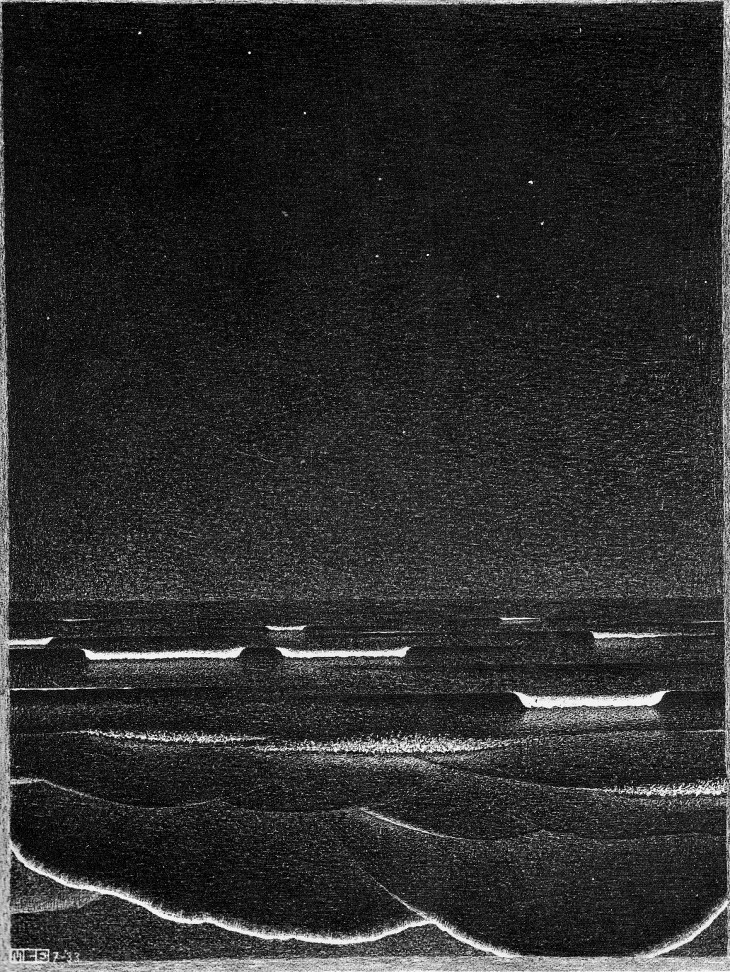
\includegraphics[scale=1.2]{escherOndas}

%----------------------------------------------------------------------------------------

\vfill % Fill the rest of the page with whitespace

\end{titlepage}

% ---------------------------------------------------------------------------------------
%         HEADER
%----------------------------------------------------------------------------------------

\fancyhead[L]{Favio Vázquez}
\fancyhead[R]{\thepage}

%----------------------------------------------------------------------------------------
\setcounter{footnote}{0}
\renewcommand*{\thefootnote}{\arabic{footnote}}
%----------------------------------------------------------------------------------------

%----------------------------------------------------------------------------------------
%%			BEGIN DOCUMENT
%----------------------------------------------------------------------------------------

\section{Problema 1. Problema 7.2 de Classical Electromagnetic Radiation
de Jackson \cite{jackson}.}

Una onda plana incidente en una interfaz de capas como se muestra en la figura. Los 
índices de refracción de los tres medios no impermeables son $n_1$, $n_2$ y $n_3$. 
El grosor de la capa intermedia es $d$. Cada uno de los otros medios es semi-infinito.

\begin{enumerate}[label=\textbf{(\alph*)}]
 \item Calcule los coeficientes de transmisión y reflexión (las tasas de del flujo de 
 Poynting transmitida y reflejada al flujo incidente), y esboce su comportamiento como 
 función de la frecuencia para $n_1 = 1$, $n_2 = 2$, $n_3 = 3$; $n_1 = 3$, $n_2 = 2$, 
 $n_3 = 1$ y $n_1 = 2$, $n_2 = 4$, $n_3 = 1$.

\begin{figure}[H]
 \center 
 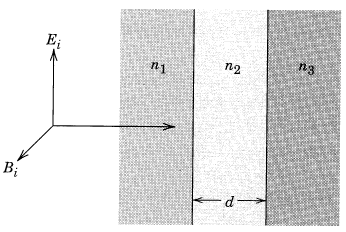
\includegraphics[scale=0.7]{problema1fig1}
\end{figure}

\item El medio $n_1$ es parte de un sistema óptico (e.g., una lente); el medio 
$n_3$ es aire $(n_3 = 1)$. Se desea colocar un revestimiento óptico (medio $n_2$) 
sobre la superficie para que no haya reflexión para ondas de frecuencia $\omega_0$. 
¿Qué grosor $d$ e índice de refracción $n_2$ son necesarios?

\end{enumerate}

\vspace{.3cm}

\underline{Solución:} \vspace{.3cm}

\textbf{(a)} Hago notar de que no encuentro una manera simple de hacer este problema, y el mecanismo 
que utilicé para solucionarlo fue inspirado en un texto que se llama ``A Companion 
to J.D. Jackson's Classical Electrodynamics'', de R. Magyar \cite{magyar}. En la 
discusión del capítulo 7 del texto de Jackson \cite{jackson}, argumenta algunas cosas interesantes que 
pueden utilizarse para resolver este problema, y aunque su discusión es mucho más 
extensa, la condensé para esta solución. Comencemos entonces.

\vspace{.3cm}

Como dice el enunciado, una onda electromagnética incide desde la izquierda y viaja 
por las capas; debido a que tratamos con una onda electromagnética sabemos que 
$\mathbf{k} \times \hat{\mathbf{n}} = 0$ y $\mathbf{B} \cdot \mathbf{E} = 0$, lo 
cual nos dice que $\mathbf{E}$ y $\mathbf{B}$ son perpendiculares al movimiento 
de la onda y son mutuamente perpendiculares entre ellas. Ya que los tres medios 
son no-permeables tenemos que $\mu_1 = \mu_2 = \mu_3 = 1$ y por lo tanto el 
índice de refracción para cara medio solo dependerá de las $\epsilon_i$. 

\vspace{.3cm}

Pensemos ahora en el recorrido de la onda por las capas. La primera capa puede reflejar 
la onda y contribuir directamente al coeficiente de reflexión efectivo, o también 
puede transmitir la onda. La segunda capa también puede reflejar la onda, si esto 
ocurre viajará de vuelta a la primera capa y puede ser transmitida a la misma. O 
la onda puede ser reflejada de vuelta. Y esto ocurre también si consideramos la 
tercera capa, por lo que vemos que el coeficiente de reflexión consistirá en una 
serie infinita de términos, donde cada término corresponde a una cierta cantidad 
de rebotes entre las capas antes de que la onda es finalmente reflejada a la 
izquierda. 

\vspace{.3cm}

Podemos escribir esto como 

\begin{equation}
r = r_{12} + t_{12}r_{23}t_{21} \euler^{2ik_2d} + t_{12}r_{23}r_{21}t_{21}
\euler^{4ik_2d} + \dots
\label{eq:reflex1}
\end{equation}

El primer término de esta ecuación corresponde a la reflexión en la interfaz 
$n_1-n_2$, el segundo término representa una onda que para por la interfaz 
$n_1-n_2$, se refleja en la interfaz $n_2-n_3$, y luego viaja de vuelta a la 
interfaz $n_1-n_2$, y así sucesivamente podemos imaginarnos los términos 
que corresponden a múltiples reflexiones internas. En esta ecuación vemos 
el cambio de fase, relacionado con $k_2 = n_2 \omega /c$, que en el primer 
término es el producto de los cambios ya que al llegar la onda va con $ikd$ y 
al devolverse va con $i(-k)(-d)$, por lo tanto el cambio total de fase será 
$2ikd$. Si escribimos la ecuación \eqref{eq:reflex1} como 

\begin{equation}
 r = r_{12} + [t_{12}r_{23}t_{21} \euler{2ik_2d}][1 + r_{23}r_{21}\euler{2ik_2d} 
 + (r_{23}r_{21})^2 \euler{4ik_2d} + \dots],
\end{equation}

y viendo que el segundo término es una serie geométrica que puede escribirse como 

\begin{equation}
 \sum_0^\infty x^n = \frac{1}{1-x},
\end{equation}

nos queda que, con $x = r_{23}r_{21}\euler^{2ik_2d}$,

\begin{equation}
 r = r_{12} + [t_{12}r_{23}t_{21} \euler^{2ik_2d}]\left[\frac{1}{1 - 
 r_{23}r_{21}\euler^{2ik_2d}} \right].
\end{equation}

De la ecuación (7.42) de Jackson \cite{jackson} vemos que 

\begin{equation}
 r_{ij} = \frac{n_i - n_j}{n_i + n_j},
\end{equation}

y 

\begin{equation}
 t_{ij} = \frac{2n_i}{n_i + n_j}.
\end{equation}

Con estas ecuaciones podemos mostrar que 

\begin{equation}
 r_{12} = \frac{n_1 - n_2}{n_1 + n_2} = - \frac{n_2 - n_1}{n_1 + n_2} = - r_{21},
\end{equation}

y que 

\begin{equation}
 t_{12}t_{21} = \left(\frac{2n_1}{n_1 + n_2} \right)\left(\frac{2n_1}{n_1 + n_2}\right) = 
 \frac{4 n_1 n_2}{(n_1 + n_2)^2} = 1 - \frac{(n_1 - n_2)^2}{(n_1 + n_2)^2} = 1 + r_{12}r_{21}.
\end{equation}

Por lo tanto podemos escribir 

\begin{equation}
 r = r_{12} + \frac{(1 + r_{12}r_{21})\euler^{2ik_2d}}{1 + r_{12}r_{23}\euler^{2ik_2d}} = 
 \frac{r_{12} + r_{23}\euler^{2ik_2d}}{1 + r_{12}r_{23}\euler^{2ik_2d}}.
\end{equation}

El coeficiente de reflexión se define como $R = |r|^2$, por lo tanto 

\begin{equation}
 \boxed{R = \frac{r_{12}^2 + r_{23}^2 + 2r_{12}r_{23}\cos{(2k_2d)}}{1 + 2r_{12}r_{23} 
 \cos{(2k_2d)} + (r_{12}r_{23})^2}},
\end{equation}

y debido a que $R + T = 1$ el coeficiente de transmisión resulta en 

\begin{equation}
 \boxed{T = \frac{1 - r_{12}^2 - r_{23}^2 + (r_{12}r_{23})^2}{1 + 2r_{12}r_{23}\cos{(2k_2d)} 
 + (r_{12}r_{21})^2}}.
\end{equation}

Necesitamos ahora hacer una serie de gráficos para el comportamiento de los índices 
de reflexión y transmisión que encontramos para distintos índices de refracción. 

\vspace{.3cm}

Si $n_1 = 1$, $n_2 = 2$ y $n_3 = 3$, haciendo $d = 1c$ nos queda 

\begin{equation}
 R = \frac{1/4 + 1/25 + 1/5\cos{4\omega}}{1 + 1/100 + 1/5\cos{4\omega}},
\end{equation}

y 

\begin{equation}
 T = \frac{1 - 1/4 - 1/25 + (1/10)^2}{1 + 1/100 + 1/5\cos{4\omega}}
\end{equation}

cuyo gráfico es 

\begin{figure}[H]
 \center 
 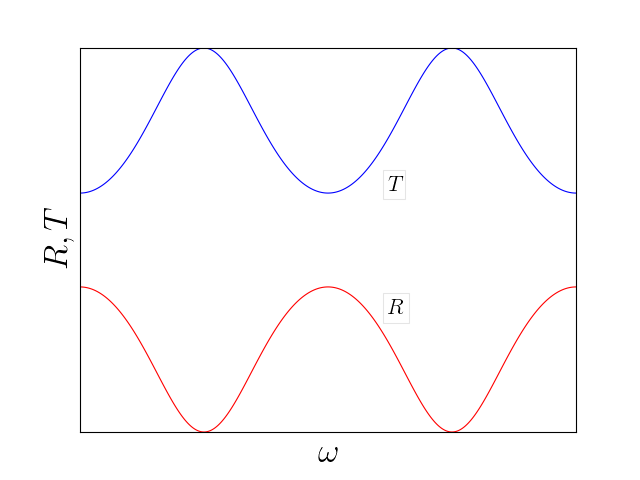
\includegraphics[scale=0.5]{problema1fig2}
 \caption{Coeficientes de reflexión y transmisión para $n_1 = 1$, $n_2 = 2$ y $n_3 = 3$.}
\end{figure}

Si $n_1 = 3$, $n_2 =2$ y $n_3 = 1$ nos queda

\begin{equation}
 R = \frac{1/4 + 1/25 + 1/5\cos{4\omega}}{1 + 1/100 + 1/5\cos{4\omega}},
\end{equation}

y 

\begin{equation}
 T = \frac{1 - 1/4 - 1/25 + (1/10)^2}{1 + 1/100 + 1/5\cos{4\omega}}
\end{equation}

cuyo gráfico es el mismo que en el anterior caso 

\begin{figure}[H]
 \center 
 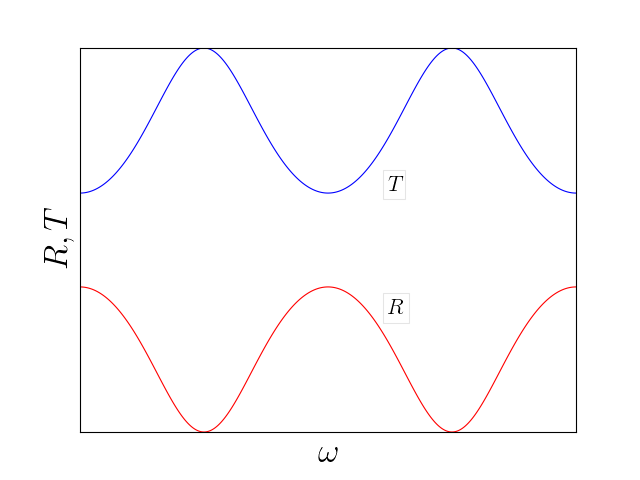
\includegraphics[scale=0.5]{problema1fig2}
 \caption{Coeficientes de reflexión y transmisión para $n_1 = 3$, $n_2 = 2$ y $n_3 = 1$.}
\end{figure}

Si $n_1 = 2$, $n_2 =4$ y $n_3 = 1$ nos queda

\begin{equation}
 R = \frac{1/9 + 9/25 - 2/5\cos{8\omega}}{1 + 1/25 - 2/5\cos{8\omega}},
\end{equation}

y 

\begin{equation}
 T = \frac{1 - 1/9 - 9/25 + 1/25}{1 + 1/25 - 2/5\cos{8\omega}}
\end{equation}

cuyo gráfico es 

\begin{figure}[H]
 \center 
 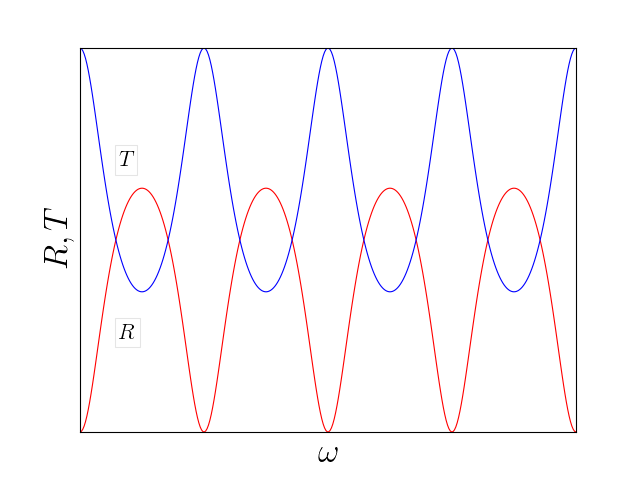
\includegraphics[scale=0.5]{problema1fig3}
 \caption{Coeficientes de reflexión y transmisión para $n_1 = 2$, $n_2 = 4$ y $n_3 = 1$.}
\end{figure}

El código para hacer estas imágenes se encuentra en un repositorio público el cual 
administro, donde también están los PDF de todas las tareas, así como el código 
\LaTeX \space con el que las hago. La página es: 
\href{https://github.com/FavioVazquez/Electrodinamica-Clasica-PCF}{https://github.com/FavioVazquez/Electrodinamica-Clasica-PCF}.
Los códigos están en NoteBooks de Python 3, los cuales GitHub renderiza de forma 
automática y pueden verse en línea.

\vspace{.3cm} 

El código que hace las primeras dos imágenes es:

\begin{lstlisting}[language=Python]
from __future__ import print_function
import numpy as np
from numpy import arccos,sin, cos, pi, array, sqrt
import matplotlib
matplotlib.use('nbagg')
import matplotlib.pyplot as plt
from matplotlib import rc

rc('font',**{'family':'sans-serif','sans-serif':['Helvetica']})
## for Palatino and other serif fonts use:
#rc('font',**{'family':'serif','serif':['Palatino']})
rc('text', usetex=True)

#LaTeX
plt.rc('text', usetex=True)
plt.rc('font', family='serif')

# Case n_1 = 1, n_2 = 2, n_3 = 3 and n_1 = 3, n_2 = 2, n_3 = 3.

# linespace for omega 
omega = np.linspace(0,pi,360)

# Def. of R and T
R_1 = (1/4 + 1/25 + 1/5*cos(4*omega))/(1 + 1/100 + 1/5*cos(4*omega))
T_1 = (1 - 1/4 - 1/25 + 1/100)/(1 + 1/100 + 1/5*cos(4*omega))

# Style
plt.ylabel(r'$R,T$', fontsize=30)
plt.xlabel(r'$\omega$',fontsize=30)
plt.xticks([])
plt.yticks([])

# Legend
plt.text(0.4, 0.33, r"$R$", bbox=dict(facecolor='white', alpha=0.1),
         fontsize=20)
plt.text(0.4, 0.65, r"$T$", bbox=dict(facecolor='white', alpha=0.1),
         fontsize=20)

# Plot
plt.plot(omega,R_1,"red",omega,T_1,"blue")
plt.show()
\end{lstlisting}

\newpage

El código que hace la segunda imagen es:

\begin{lstlisting}[language=Python]
from __future__ import print_function
import numpy as np
from numpy import arccos,sin, cos, pi, array, sqrt
import matplotlib
matplotlib.use('nbagg')
import matplotlib.pyplot as plt
from matplotlib import rc

rc('font',**{'family':'sans-serif','sans-serif':['Helvetica']})
## for Palatino and other serif fonts use:
#rc('font',**{'family':'serif','serif':['Palatino']})
rc('text', usetex=True)

#LaTeX
plt.rc('text', usetex=True)
plt.rc('font', family='serif')

# Case n_1 = 2, n_2 = 4, n_3 = 1

# linespace for omega 
omega = np.linspace(0,pi,360)

# Def. of R and T
R_2 = (1/9 + 9/25 - 2/5*cos(8*omega))/(1 + 1/25 - 2/5*cos(8*omega))
T_2 = (1 - 1/9 - 9/25 + 1/25)/(1 + 1/25 - 2/5*cos(8*omega))

# Style
plt.ylabel(r'$R,T$', fontsize=30)
plt.xlabel(r'$\omega$',fontsize=30)
plt.xticks([])
plt.yticks([])

# Legend
plt.text(0.25, 0.3, r"$R$", bbox=dict(facecolor='white', alpha=0.1),fontsize=20)
plt.text(0.25, 0.65, r"$T$", bbox=dict(facecolor='white', alpha=0.1),fontsize=20)

# Plot
plt.plot(omega,R_2,"red",omega,T_2,"blue")
plt.show()
\end{lstlisting}

\textbf{(b)} Si $n_3 = 1$ el índice de reflexión se reduce a 

\begin{equation}
 R = 1 - \frac{8n_1 n_2^2}{n_1^2 + [1 + n_1(4 + n_1)]n_2^2 + n_2^4 + 
 (n_1 - n_2)(n_1 + n_2)(n_2^2 - 1)\cos{(2 d n_2 \omega_0)}}
\end{equation}

donde hemos cambiado $\omega$ por $\omega_0$ como lo especifica el inciso. Ahora 
si podemos hacer que $\cos{(2 d n_2 \omega_0)} = -1$ el requerimiento de que $R = 0$ 
se reduce a 

\begin{equation}
 n_1^2 + [1 + n_1(4 + n_1)]n_2^2 + n_2^4 + 
 (n_1 - n_2)(n_1 + n_2)(n_2^2 - 1) - 8n_1 n_2^2 = 0,
\end{equation}

lo que implica que $n_2 = \sqrt{n_1}$. Por lo tanto para que se cumpla que $R=0$, debemos 
escoger $n_2 = \sqrt{n_1}$ y para que se cumpla la condición que impusimos en el 
coseno, debe tenerse que $d = (m - 1/2)\frac{\pi}{\sqrt{n\omega_0}}$.

\newpage

\section{Problema 2. Problema 7.3 de Classical Electromagnetic Radiation
de Jackson \cite{jackson}.}

Dos losas planas semi-infinitas con el mismo dieléctrico sin pérdidas, uniformidad,
isotropía, no-permeabilidad con índice de refracción $n$ son paralelas, y están 
separadas por una brecha de aire ($n = 1$) de ancho $d$. Una onda electromagnética 
de frecuencua $\omega$ incide en la brecha desde una de las losas con un ángulo 
de incidencia $i$. Para una polarización lineal tanto paralela como perpendicular 
al plano de incidencia,

\begin{enumerate}[label=\textbf{(\alph*)}]
 \item calcule la tasa de potencia transmitida a la segunda losa con respecto 
 al poder incidente y la tasa de poder reflejado con respecto al incidente;
 \item para un $i$ mayor que el ángulo crítico para reflexión interna total, 
 esboce la tasa de potencia transmitida con respecto a la potencia incidente 
 como una función de $d$ medido en unidades de longitud de onda en la brecha.
\end{enumerate}

\vspace{.3cm}

\underline{Solución:} \vspace{.3cm}

\newpage

\section{Problema 3. Problema 7.5 de Classical Electromagnetic Radiation
de Jackson \cite{jackson}.}

Una onda electromagnética polarizada $\mathbf{E} = \mathbf{E}_i \euler^{i\mathbf{k}} 
\cdot \mathbf{x} - i\omega t$ incide normalmente sobre una lámina plana uniforme 
de una excelente conducción ($\omega \gg \omega \epsilon_0$) con un grosor de $D$. 
Asumiendo que en el espacio y en la lámina conductora $\mu/\mu_0 = \epsilon/\epsilon_0 
= 1$, discuta la reflexión y transmisión de la onda incidente. 

\begin{enumerate}[label=\textbf{(\alph*)}]
 \item Muestre que las amplitudes de las onda reflejada y transmitida, correctas 
 a primer orden en $(\epsilon_0 \omega /\sigma)^1/2)$, son 
 
 $$
 \frac{E_r}{E_i} = \frac{-(1 - \euler^{-2\lambda})}{(1 - \euler^{-2\lambda}) 
 + \gamma(1 + \euler^{-2\lambda})}
 $$
 
  $$
 \frac{E_t}{E_i} = \frac{2\gamma \euler^{-\lambda}}{(1 - \euler^{-2\lambda}) 
 + \gamma(1 + \euler^{-2\lambda})}
 $$
 
 donde 
 
 $$
 \gamma = \sqrt{\frac{2\epsilon_0 \omega}{\sigma}}(1 - i) = \frac{\omega \delta}{c}
 (1 - i)
 $$
 
 $$
 \lambda = (1-i)D/\delta
 $$
 
  y $\delta = \sqrt{2/\omega \mu \sigma}$ es la profundidad de penetración.
 
 \item Verifique que para un grosor igual a cero y un grosor infinito se obtienen 
 los resultados limitantes apropiados.
 \item Muestre que, excepto para láminas de muy poco grosor, el coeficiente de 
 transmisión es 
 
 $$
 T = \frac{8(\text{Re} \gamma)^2 \euler^{-2D/\gamma}}{1 - 2\euler^{-2D/\gamma} 
 \cos{2D/\delta) + \euler^{-4/\gamma}}}
 $$
\end{enumerate}

Esboce log $T$ como una función de $(D/\delta)$, asumiendo que Re $\gamma = 10^{-2}$. 
Defina ``grosor muy pequeño''.

\vspace{.3cm}

\underline{Solución:} \vspace{.3cm}

\newpage

\section{Problema 4. Problema 7.14 de Classical Electromagnetic Radiation
de Jackson \cite{jackson}. (Es el 7.9 de la 2da ed.)}

Un modelo simple para la propagación de ondas de radio en la atmósfera de la 
Tierra o ionosfera consiste en una tierra plana en $z = 0$ y un medio no 
uniforme con $\epsilon = \epsilon(z)$ para $z > 0$. Considere la ecuaciones 
de Maxwell bajo la suposición de que los campos son independientes de $y$ y 
pueden escribirse como funciones de $z$ por $\euler^{i(kx - \omega t)}$. 

\begin{enumerate}[label=\textbf{(\alph*)}]
 \item Muestre que la ecuación de onda que gobierna la propagación para $z > 0$ 
 es 
 
 $$
 \frac{d^2 F}{dz^2} + q^2(z) F = 0,
 $$
 
 donde 
 
 $$
 q^2(z) = \omega^2 \mu_0 \epsilon(z) - k^2
 $$
 
 y $F = E_y$ para la polarización \emph{horizontal}, y 
 
 $$
 q^2(z) = \omega^2 \mu_0 \epsilon(z) + \frac{1}{2\epsilon}\frac{d^2 \epsilon}{dz^2} 
 - \frac{3}{4\epsilon^2}\left(\frac{d \epsilon}{d z} \right)^2 - k^2
 $$
 
 con $F = \sqrt{\epsilon/\epsilon_0}E_z$ para la polarización \emph{vertical}.
 
 \item Use la aproximación WKB para tratar la propagación de ondas dirigidas 
 verticalmente hacia la ionosfera ($k = 0$), asumiendo que la constante dieléctrica 
 está dad por (7.59) con una frecuencia de plasma $\omega_p(z)$ gobernada por una 
 densidad electrónica como se muestra en la figura 7.11. Verifique que los argumentos 
 cualitativos de la sección 7.6 se mantienen, con discrepancias en detalle solo 
 para $\omega ~ \omega_{p,\text{max}}$.
 
 \item Usando los resultados WKB de la parte (b) y los conceptos de propagación 
 de un pulso de la sección 7.8, define una altura efectiva de la ionosfera $h'(\omega)$ 
 calculando el tiempo $T$ para un pulso de frecuencia dominante $\omega$ que viaja 
 hacia arriba y se refleja ($h' \equiv cT/2)$. [La aproximación WKB es discutida 
 en la mayoría de los libros de mecánica cuántica].
\end{enumerate}

\vspace{.3cm}

\underline{Solución:} \vspace{.3cm}

\newpage

\begin{thebibliography}{10}
\bibitem{jackson}
J. Jackson, \emph{Classical Electrodynamics}, 3ra edición. John Wiley and Sons, Inc. 
1999.
\bibitem{magyar}
R. Magyar, \emph{A Companion to Classical Electrodynamics 3rd Edition by J.D. 
Jackson}, 2001.
\bibitem{griffiths}
D. Griffiths, \emph{Indtroduction to Electrodynamics}, 4ta edición. Pearson, 2013.
\end{thebibliography}

\end{document}